\section{Results}\label{sec:results}

All numbers in this section come from the base, untuned gpt-oss-120b model
against the frozen 30-spec holdout, three seeds per arm unless stated
otherwise. Every run reported here is gate-check clean: 0
\texttt{api\_error} rows, 0 unextracted rows.

\BfPara{Headline Comparison} Framing L solves 18, 16, and 18 of 30 specs
across its three seeds (mean 17.3, 571--616 model calls per run). Framing A
solves 12, 8, and 12 (mean 10.7, 960--990 model calls per run). The ranges do
not overlap: framing L's worst seed (16) exceeds framing A's best seed (12).
\autoref{fig:fig_seeds} plots solved specs per seed for both arms alongside
mean model calls.

\begin{figure*}[t]
\centering
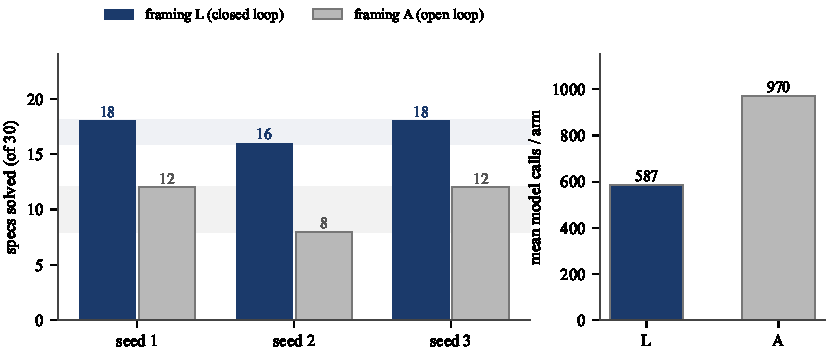
\includegraphics[width=\textwidth]{figures/fig_seeds.pdf}
\caption{Solved specs per seed for framing L and framing A, with mean model
calls per run. The three seeds of each arm are independent runs, not paired
with one another or across arms.}\label{fig:fig_seeds}\end{figure*}

Applying the pre-registered rule from \autoref{sec:method} to a single
pairing illustrates why all nine pairings are required rather than one.
Loop seed 1 against the same-session open-loop control is $+6$ specs,
$p{=}0.031$, a win. Loop seed 2 against the same control is $+4$ specs,
$p{=}0.125$, null by the rule. Reporting seed 1 alone would have been a
sampling accident in the favorable direction.

\BfPara{Pairwise Comparison} \autoref{tab:pairings} gives all nine (loop
seed, open seed) pairings. The delta ranges from $+4$ to $+10$ specs. One
spec is lost across all nine pairings combined (spec 181, in two of the
three pairings against loop seed 3), and no pairing shows a net loss.
Sign-test $p$ ranges from 0.0020 to 0.1250 depending on which two seeds are
compared.

\begin{table}[t]
\centering
\small
\caption{All nine (loop seed, open seed) pairings, base gpt-oss-120b,
30-spec holdout. Loop seeds solve 18/16/18; open seeds solve 12/8/12. Gained
and lost count specs relative to the paired open-loop seed; $p$ is the exact
sign-test $p$-value for that pairing.}
\label{tab:pairings}
\begin{tabular}{@{}ccrrrr@{}}
\toprule
L & A & $\Delta$ & Gain & Loss & $p$ \\
\midrule
1 & 1 & +6  & 6  & 0 & 0.0313 \\
1 & 2 & +10 & 10 & 0 & 0.0020 \\
1 & 3 & +6  & 6  & 0 & 0.0313 \\
2 & 1 & +4  & 4  & 0 & 0.1250 \\
2 & 2 & +8  & 8  & 0 & 0.0078 \\
2 & 3 & +4  & 4  & 0 & 0.1250 \\
3 & 1 & +6  & 7  & 1 & 0.0703 \\
3 & 2 & +10 & 11 & 1 & 0.0063 \\
3 & 3 & +6  & 6  & 0 & 0.0313 \\
\bottomrule
\end{tabular}
\end{table}

\BfPara{Per-Spec Stability} Only two specs, 13 and 15, are solved by framing
L in every seed and by framing A in none. Specs 132 and 191 are loop-solved
in 2 of 3 seeds and never solved open-loop. Specs 32, 106, 133, and 174 are
loop-solved in 1 of 3 seeds and never solved open-loop. No spec is ever
open-loop-only: framing A never solves a spec that framing L fails on every
seed. \autoref{fig:fig_perspec} shows the per-spec solve rate over seeds for
both arms. The loop reliably adds specs in the five-to-seven range per seed,
but which specs it adds varies by seed; the effect is a larger reachable
set, not a fixed, deterministic gain.

\begin{figure*}[t]
\centering
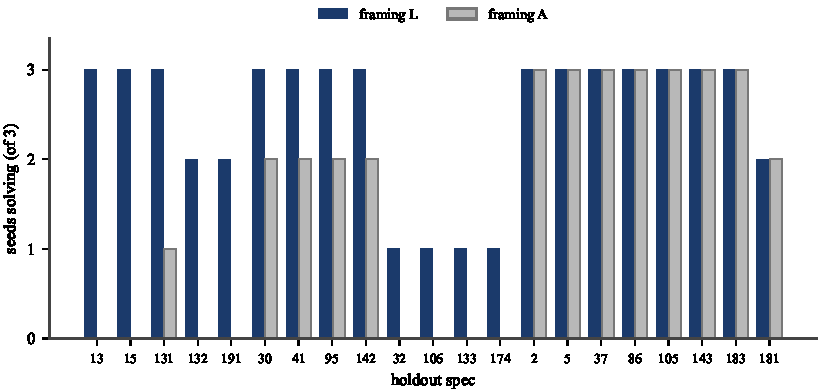
\includegraphics[width=\textwidth]{figures/fig_perspec.pdf}
\caption{Per-spec solve rate over the three seeds of each arm, framing L
against framing A.}\label{fig:fig_perspec}\end{figure*}

\BfPara{Mechanism} Loop seed 1 carries per-call provenance for every solved
spec. Of its 18 solves, 9 came from a fresh generation in round 0 (the first
of the 8 independent draws) and 9 came from a later, repair round. Restricting
to the 6 specs gained relative to the frozen open-loop control (13, 15, 106,
174, 181, 191), 5 of the 6 were won on a repair round: three entered the
repair prompt at the \texttt{sany} rung (specs 13, 106, 174) and two at the
\texttt{tlc\_error} rung (specs 15, 191). Only spec 181 was solved on the
first round-0 draw. The advantage over the open-loop control is concentrated
in the repair mechanism, not in round-0 sampling diversity.

\BfPara{Confound Checks} Two confounds were closed before reporting the
headline numbers. First, endpoint drift: the frozen open-loop control was
measured months before framing L. Re-running the open-loop control on the
same warm endpoint at a matched 32-call budget reproduced 12/30 exactly.
Per-sample SANY rate across that session, in run order, was 16.6\%, 22.9\%,
23.9\%, 25.7\%, 15.2\%, with median per-sample latency 20.3s, 23.0s, 22.6s,
22.7s, 20.2s; the third open-loop seed's 8/30 is spec-level sampling noise on
a stable serve, not a degrading endpoint. Second, single-seed accident: three
seeds per arm were run and all three are reported for both arms, not a
subset chosen after the fact.

Per-sample pass rate is not comparable across the two framings. Framing L stops a spec on its first passing draw, so an easy spec
contributes exactly one passing row to the framing-L pool while framing A can
bank 20 or more passing rows on the same spec across its $k{=}32$ draws.
Per-sample pass rate is therefore structurally biased against framing L
(3.0\% vs.\ 7.5\%) and is not a capability comparison between the arms.
Per-sample SANY rate carries the same bias in the same direction, which makes
framing L's advantage there conservative rather than inflated: 24.1\%
(bootstrap 95\% CI [22.2, 26.1]) against 14.1\% (bootstrap 95\% CI [12.8,
15.3]), pooled over 1,760 and 2,910 rows respectively.

\BfPara{Reachability Ceiling} Pooling all six arms (4,670 draws total), 834
draws (18\%) pass SANY, 678 (15\%) additionally satisfy the \texttt{.cfg}
signature, and 219 (5\%) pass TLC. \autoref{fig:fig_funnel} shows this funnel
per draw and per spec. At the spec level, coverage is wider than the
per-draw rate suggests: all 30 holdout specs produce at least one parsing
candidate somewhere across the six arms, 26 of 30 produce at least one
signature-complete candidate, and 20 of 30 produce at least one TLC pass. The
worst spec by density is 106, with 1 passing draw out of 174; the best is
181, with 101 out of 158. Spec-level SANY coverage is already 100\%: the
ceiling on solvable specs is set by TLC and signature completion, not by
parsing.

\begin{figure*}[t]
\centering
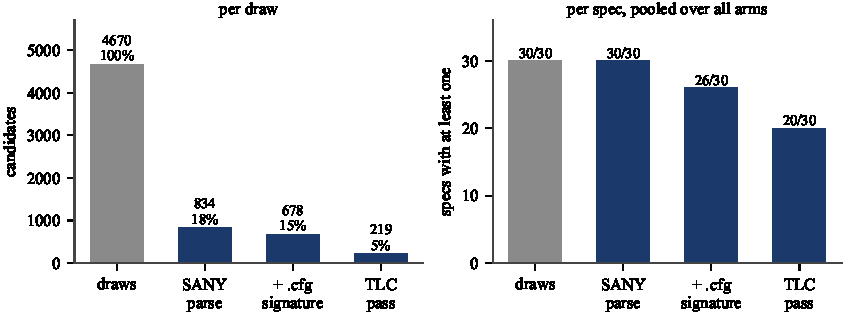
\includegraphics[width=\textwidth]{figures/fig_funnel.pdf}
\caption{Draws, SANY parse, \texttt{.cfg} signature completion, and TLC
pass, pooled over all six arms and broken out per draw and per
spec.}\label{fig:fig_funnel}\end{figure*}

\BfPara{Failure Taxonomy} 3,836 SANY failures were classified across the six
arms. Grammar failures (the module does not parse) account for 1,967 (51\%);
unknown-operator errors account for 1,304 (34\%); the remainder splits across
an unclassified other category (375, 10\%), duplicate definitions (97, 3\%),
wrong arity (86, 2\%), and missing substitution or level errors (7, 0\%).
\autoref{fig:fig_taxonomy} breaks down both the top-level classes and the
unknown-operator subclasses.

\begin{figure*}[t]
\centering
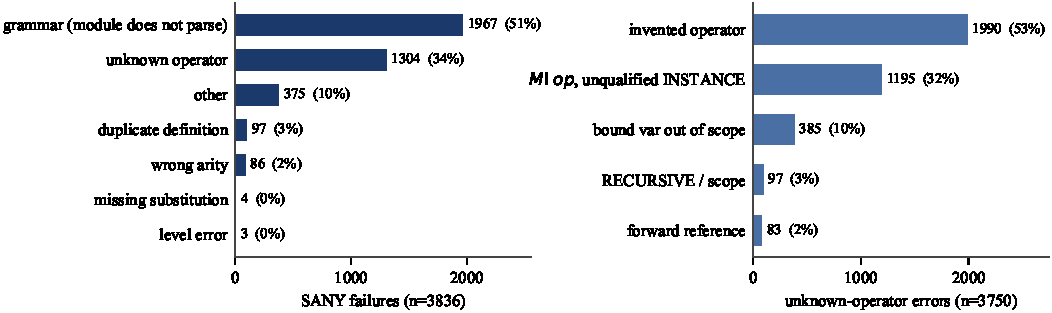
\includegraphics[width=\textwidth]{figures/fig_taxonomy.pdf}
\caption{SANY failure classes across the six arms, and the breakdown of the
unknown-operator class into its five subtypes.}\label{fig:fig_taxonomy}\end{figure*}

Of 3,750 unknown-operator errors located in the candidate's own module, 1,990
(53\%) reference an operator that exists nowhere in the module or its
imports, 1,195 (32\%) qualify a name against an unqualified
\texttt{INSTANCE}, 385 (10\%) are a bound variable escaping its quantifier's
scope, 97 (3\%) use \texttt{RECURSIVE} without a preceding declaration, and
83 (2\%) are a genuine forward reference. The \texttt{INSTANCE} case is one
misunderstanding that produces two error classes at once: the model writes
an unqualified \texttt{INSTANCE Bakery}, which imports every name from
\texttt{Bakery} directly, and then separately writes
\texttt{vars == Bakery!vars}, a qualified reference that requires a named
instance; the redefinition then collides with the name the unqualified
\texttt{INSTANCE} already imported. The five most frequent offending tokens
in the parse-failure population are \texttt{:} (139), \texttt{\textbackslash
subseteq} (126), \texttt{,} (118), \texttt{AS} (89), and \texttt{LET} (85),
corresponding respectively to comma-separated \texttt{LET} bindings,
\verb|\E x \subseteq S|, \texttt{INSTANCE M AS B}, lowercase
\texttt{let\ldots in}, and \verb|\Sum i \in S :|. Each is a construct
borrowed from a more common programming language.

\BfPara{Lint Negative Result} A deterministic lint pass (drop declarations
that collide with an \texttt{EXTENDS}, add a missing standard-module
\texttt{EXTENDS}, drop duplicate definitions) was applied to the unsolved
specs. It recovered 88 candidates across 9 specs from fail-to-parse to
parsing. Specs flipped from unsolved to solved by this pass: zero. All 88
recovered candidates subsequently failed at TLC. Forcing output to parse, on
its own, does not translate into a solved spec.

\BfPara{Fine-Tuning Comparison} The best fine-tuned checkpoint measured in
this program reaches 15/30 open-loop against a base-model control of 12/30:
$+3$ specs, 5 gained, 2 lost, McNemar exact $p{=}0.45$, null by the
pre-registered rule. The untuned base model inside the loop (mean 17.3/30)
exceeds this fine-tuned checkpoint's open-loop score. The 15/30 also
decomposes further: 4 of those specs are library modules scored on SANY
alone, 1 is a proof module scored on TLAPS, leaving 10 specs actually
model-checked by TLC.

\BfPara{Grammar Measurement} \gfile{} was scored against
438 known-good specs (the examples corpus plus the 30-spec holdout) and 1,543
measured real parse failures. It clears the false-reject gate: 0 of the 438
known-good specs are rejected. Against real failures it rejects 1,338 of
1,543 (86.7\%). The structural precursor already in the repository,
\texttt{tla\_module\_v0.ebnf}, false-rejects 5.0\% of the known-good specs
and catches 3.2\% of real parse failures; because the candidates are already
100\% well-framed, balanced, and terminated, the structural tier has almost
nothing left to act on. A companion \texttt{.cfg} grammar false-rejects 0 of
230 corpus configuration files. \autoref{fig:fig_grammar} compares the two
module-grammar versions on false-reject rate and catch rate.

\begin{figure}[t]\centering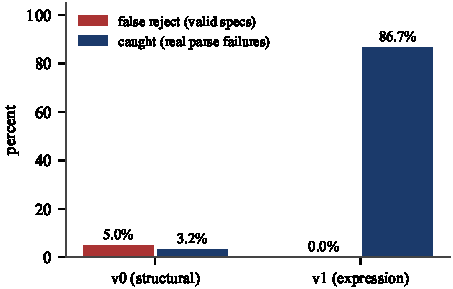
\includegraphics[width=\linewidth]{figures/fig_grammar.pdf}
\caption{Grammar v0 against v1: false-reject rate on the 438-spec known-good
corpus and catch rate on 1,543 measured parse failures.}\label{fig:fig_grammar}\end{figure}

The constructs that forced grammar iteration, none of them guessable from a
language reference alone, include nested junction lists under a single
bullet, bare \verb|\| as set difference, postfix application \texttt{f[x]},
\verb|\leq| and \verb|\geq|, operator symbols passed as arguments
(\texttt{Fold(+, 0, ...)}), tuple subscripts in \verb|[][Next]_<<a,b>>|,
qualification after an application (\texttt{P(Succ)!Reachable0}), the
parenthesised infix operators \texttt{(+)}, \texttt{(-)}, \texttt{(\textbackslash
X)}, the symbolic operator set \texttt{\^{}\^{} ** ++ -- // \%\% \#\# \$\$ ??
!!}, \texttt{RECURSIVE} declared inside a \texttt{LET}, nested
\texttt{---- MODULE Inner ----} units, nesting block comments
\texttt{(* (* *) *)}, subexpression labels \texttt{P0 :: expr}, and
identifiers beginning with a digit (\texttt{---- MODULE 2PCwithBTM ----} is a
real corpus spec). Junction-list alignment is not enforced by either grammar
version and is not addressable by a context-free grammar: it is
context-sensitive, and SANY itself uses a custom lexer for it rather than its
context-free rules.
